% ============================================================================
%  CHƯƠNG 3. CÀI ĐẶT, THỰC NGHIỆM VÀ ỨNG DỤNG
% ============================================================================
\chapter{Cài đặt, thực nghiệm và ứng dụng}\label{chap:3}

Chương này kiểm nghiệm bằng thực nghiệm các kết quả của Chương~\ref{chap:2} và trả lời bốn câu hỏi nghiên cứu nêu ở Mở đầu. Sau phần cài đặt (\cref{sec:impl}), dữ liệu hai chiều được dùng để quan sát trực tiếp biên quyết định (\cref{sec:exp2d}). \Cref{sec:benchmark} tái hiện một thí nghiệm của bài báo gốc và so sánh PWL-SVM với sáu phương pháp khác trên mười bộ dữ liệu chuẩn; \cref{sec:cost} đo chi phí tính toán; \cref{sec:application} áp dụng PWL-SVM cho bài toán dự báo vỡ nợ thẻ tín dụng; \cref{sec:discussion} thảo luận các kết quả.

% ----------------------------------------------------------------------------
\section{Cài đặt}\label{sec:impl}

Toàn bộ thực nghiệm được cài đặt bằng Python~3 với NumPy~\cite{harris2020}, SciPy~\cite{virtanen2020} và scikit-learn~\cite{pedregosa2011}. Mô-đun chính \texttt{pwlsvm.py} gồm hai lớp theo giao diện \texttt{fit}/\texttt{predict} của scikit-learn, nhờ đó dùng được trực tiếp các công cụ kiểm định chéo và tìm kiếm tham số của thư viện này. Lớp \texttt{PWLFeatures} tính ánh xạ~\eqref{eq:feature-map} cho ba dạng cộng tính, HH và GHH theo Mục~\ref{sec:maps}, với hai tùy chọn bổ sung: đặt nút theo phân vị (\cref{rem:quantile}) và chuẩn hóa $\|p\|_2=1$ (\cref{rem:scale}). Lớp \texttt{PWLSVM} chuẩn hóa từng thành phần về $[0,1]$, tính $\varphi(x)$ rồi giải bài toán tuyến tính trên $\varphi(x)$ (\cref{alg:pwlsvm}). PWL-LS-SVM được giải trực tiếp ở dạng gốc theo \cref{prop:ridge}. PWL-C-SVM có hai bộ giải: LIBSVM~\cite{chang2011} giải đúng bài toán đối ngẫu~\eqref{eq:pwl-c-dual} và được dùng cho các thí nghiệm nhỏ ở \cref{sec:exp2d,sec:cosexp}; LIBLINEAR~\cite{fan2008} giải bài toán trên đặc trưng tường minh bằng phương pháp hạ theo tọa độ, nhanh hơn nhiều khi $N$ hoặc $\gamma$ lớn, nên được dùng cho mọi thí nghiệm còn lại, với cái giá là hệ số chặn bị chính quy hóa nhẹ (nó được đưa vào như trọng số của một đặc trưng hằng bằng $10$, tương đương phạt thêm $w_0^2/200$). Mô-đun \texttt{pwlsvm\_monotone.py} bổ sung ràng buộc đơn điệu (Mục~\ref{sec:monotone}). Mọi phương pháp đối chứng được đặt trong cùng một khung, dùng chung cách chuẩn hóa, cách chia dữ liệu và cách chọn tham số.

\begin{algorithm}[t]
\caption{Huấn luyện và dự đoán với PWL-SVM}\label{alg:pwlsvm}
\begin{algorithmic}[1]
\Require dữ liệu $\{(x_k,y_k)\}_{k=1}^{N}$; dạng ánh xạ (cộng tính, HH hoặc GHH); số đặc trưng trên mỗi chiều $M/n$; hằng số $\gamma$
\Ensure trọng số $w\in\R^M$, hệ số chặn $w_0$, tham số của ánh xạ và của phép chuẩn hóa
\State Chuẩn hóa từng thành phần của $x_k$ về $[0,1]$; lưu giá trị nhỏ nhất và lớn nhất
\If{dạng cộng tính}
  \State đặt $S=M/n$ và các nút $q=s/S$ ($s=1,\dots,S-1$), hoặc các phân vị mức $s/S$, trên mỗi trục
\Else
  \For{$m=n+1,\dots,M$}
    \State sinh $1$ siêu phẳng (HH) hoặc $n$ siêu phẳng (GHH) theo~\eqref{eq:random-plane}
  \EndFor
\EndIf
\State Lập ma trận $\Phi\in\R^{N\times M}$ có hàng thứ $k$ là $\varphi(x_k)^\T$, theo~\eqref{eq:feature-map}
\State Giải~\eqref{eq:pwl-c-dual} rồi tính $w=\sum_k\alpha_ky_k\varphi(x_k)$ (PWL-C-SVM), hoặc giải~\eqref{eq:ridge} (PWL-LS-SVM)
\State \textbf{Dự đoán} điểm mới $x$: chuẩn hóa $x$ bằng các giá trị đã lưu, trả về $\sgn\bigl(w^\T\varphi(x)+w_0\bigr)$
\end{algorithmic}
\end{algorithm}

\paragraph{Kiểm chứng tính đúng đắn.} Trên dữ liệu hai mặt trăng ($N=400$, $M=20$, $\gamma=10$), với cả ba dạng ánh xạ, hai hệ thức của Chương~\ref{chap:2} được kiểm tra bằng số. Với PWL-LS-SVM, nghiệm của dạng gốc (\cref{prop:ridge}) và nghiệm của hệ đối ngẫu~\eqref{eq:pwl-ls-dual} sai khác không quá $7\cdot10^{-12}$. Với PWL-C-SVM, vectơ $w=\sum_k\alpha_ky_k\varphi(x_k)$ khôi phục từ nghiệm đối ngẫu với hạt nhân hữu hạn hạng~\eqref{eq:kernel} trùng với vectơ thu được khi giải trực tiếp trên $\varphi(x)$ (sai khác dưới $2\cdot10^{-12}$), và hai bộ phân loại dự đoán giống hệt nhau trên toàn bộ tập kiểm tra. Ví dụ hai mặt trăng ở Mục~\ref{sec:maps} cũng tái hiện đúng hiện tượng mà bài báo gốc mô tả: bốn đặc trưng cộng tính cho một biên ba đoạn với các điểm gãy nằm trên hai đường $x(2)=\tfrac13$ và $x(2)=\tfrac23$.

% ----------------------------------------------------------------------------
\section{Thực nghiệm minh họa trên dữ liệu hai chiều}\label{sec:exp2d}

Dữ liệu hai chiều cho phép nhìn trực tiếp biên quyết định. Đề án dùng bốn bộ dữ liệu tổng hợp có độ khó tăng dần (\cref{fig:demo2d}): hai mặt trăng (nhiễu Gauss với độ lệch chuẩn $0{,}15$), hai vòng tròn đồng tâm (tỉ số bán kính $0{,}5$, nhiễu $0{,}08$), bàn cờ $4\times4$ và hai xoắn ốc lồng nhau ($1{,}6$ vòng, nhiễu $0{,}06$); mỗi bộ gồm $500$ điểm huấn luyện và $500$ điểm kiểm tra như trong bài báo gốc. Năm phương pháp được so sánh: SVM tuyến tính; PWL-C-SVM với ánh xạ cộng tính ($M/n=10$), HH ($M/n=50$, tức $98$ siêu phẳng) và GHH ($M/n=25$, tức $48$ đặc trưng với tổng cộng $96$ siêu phẳng); và SVM hạt nhân Gauss. Hằng số $\gamma$ được chọn trong $\{2^{-3},2^{-1},\dots,2^{11}\}$ bằng kiểm định chéo $5$ phần trên tập huấn luyện (với SVM hạt nhân Gauss, $1/\sigma^2$ được chọn đồng thời trong $\{2^{-3},2^{-1},\dots,2^{9}\}$), và toàn bộ quy trình được lặp lại $10$ lần (\cref{tab:exp2d}).

\begin{figure}[t]
\centering
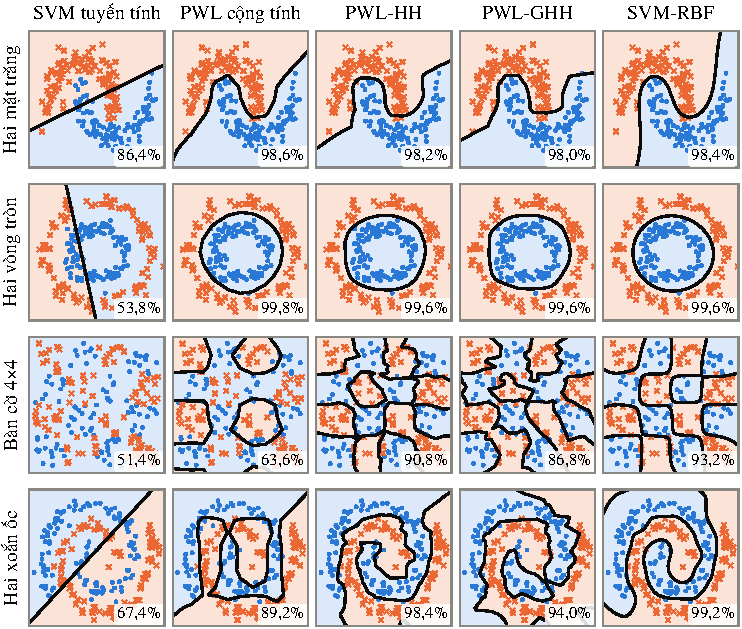
\includegraphics[width=0.8\linewidth]{fig_demo_2d.pdf}
\caption[Biên quyết định của năm phương pháp trên dữ liệu hai chiều]{Biên quyết định của năm phương pháp trên bốn bộ dữ liệu hai chiều (lần lặp đầu tiên). Chấm xanh và dấu nhân cam là các điểm kiểm tra của hai lớp; con số ở góc là độ chính xác trên $500$ điểm kiểm tra.}
\label{fig:demo2d}
\end{figure}

\begin{table}[t]
\centering
\caption[Độ chính xác trên dữ liệu hai chiều]{Độ chính xác trên tập kiểm tra (\%, trung bình $\pm$ độ lệch chuẩn qua $10$ lần lặp) trên dữ liệu hai chiều; in đậm là giá trị trung bình cao nhất mỗi hàng.}
\label{tab:exp2d}
\small
\renewcommand{\arraystretch}{1.2}
\setlength{\tabcolsep}{4pt}
\begin{tabular}{@{}l c c c c c@{}}
\toprule
\textbf{Dữ liệu} & \textbf{SVM tuyến tính} & \textbf{PWL cộng tính} & \textbf{PWL-HH} & \textbf{PWL-GHH} & \textbf{SVM-RBF}\\
\midrule
Hai mặt trăng & $87{,}3\pm2{,}0$ & $98{,}8\pm0{,}7$ & $98{,}7\pm0{,}7$ & $98{,}6\pm0{,}8$ & $\mathbf{98{,}9}\pm0{,}6$\\
Hai vòng tròn & $52{,}7\pm3{,}5$ & $\mathbf{99{,}9}\pm0{,}1$ & $99{,}8\pm0{,}2$ & $99{,}8\pm0{,}2$ & $99{,}8\pm0{,}2$\\
Bàn cờ $4\times4$ & $50{,}0\pm2{,}4$ & $55{,}5\pm3{,}4$ & $90{,}6\pm2{,}2$ & $85{,}7\pm2{,}5$ & $\mathbf{94{,}8}\pm1{,}2$\\
Hai xoắn ốc & $64{,}8\pm2{,}7$ & $89{,}2\pm1{,}5$ & $98{,}2\pm0{,}6$ & $96{,}7\pm1{,}4$ & $\mathbf{99{,}2}\pm0{,}4$\\
\bottomrule
\end{tabular}
\end{table}

Kết quả phù hợp với phân tích ở Mục~\ref{sec:maps}. SVM tuyến tính thất bại trên cả bốn bộ, với độ chính xác xấp xỉ $50\%$ trên hai vòng tròn và bàn cờ; cả ba dạng PWL-SVM đều cải thiện rõ rệt và ngang SVM hạt nhân Gauss trên hai mặt trăng và hai vòng tròn. Ánh xạ cộng tính gần như tuyệt đối trên hai vòng tròn ($99{,}9\%$) nhưng gần như thất bại trên bàn cờ ($55{,}5\%$). Nguyên nhân nằm ở cấu trúc của mô hình chứ không ở số đặc trưng: biên $x(1)^2+x(2)^2=r^2$ của hai vòng tròn là tổng của hai hàm một biến, còn cấu trúc kiểu bàn cờ thì không mô hình cộng tính nào xử lý được, như mệnh đề sau chỉ ra.

\begin{proposition}\label{prop:xor}
Cho $a\neq b$ và $c\neq d$. Giả sử hai điểm $(a,c)$ và $(b,d)$ thuộc lớp $+1$, còn hai điểm $(a,d)$ và $(b,c)$ thuộc lớp $-1$. Khi đó không tồn tại hai hàm $g_1,g_2:\R\to\R$ nào sao cho hàm cộng tính $f(x)=g_1\bigl(x(1)\bigr)+g_2\bigl(x(2)\bigr)$ phân loại đúng cả bốn điểm.
\end{proposition}

\begin{proof}
Nếu có, thì $f(a,c)+f(b,d)>0$ và $f(a,d)+f(b,c)<0$. Nhưng cả hai tổng đều bằng $g_1(a)+g_1(b)+g_2(c)+g_2(d)$, mâu thuẫn.
\end{proof}

Bàn cờ $4\times4$ chứa rất nhiều bộ bốn điểm như vậy, nên mọi bộ phân loại cộng tính, dù dùng bao nhiêu đặc trưng, đều mắc nhiều lỗi. Kết luận này áp dụng cả cho SVM hạt nhân giao, vốn cũng là một mô hình cộng tính (Mục~\ref{sec:relations}), và giải thích vì sao trong bài báo gốc, SVM hạt nhân giao chỉ đạt $48{,}8\%$ trên dữ liệu bàn cờ~\cite[Bảng~1]{huang2013}. Hai dạng HH và GHH, với các siêu phẳng có hướng tùy ý, xử lý được cả bàn cờ lẫn xoắn ốc, dù vẫn kém SVM hạt nhân Gauss vài điểm phần trăm và cho biên gấp khúc thay vì trơn. Với cùng số siêu phẳng, GHH kém HH một chút vì số trọng số được học chỉ bằng một nửa ($50$ so với $100$): khả năng biểu diễn tổng quát của GHH (\cref{cor:boundary}) không tự động chuyển thành độ chính xác khi các siêu phẳng được sinh ngẫu nhiên.

% ----------------------------------------------------------------------------
\section{Thực nghiệm trên dữ liệu chuẩn}\label{sec:benchmark}
% ----------------------------------------------------------------------------
%  3.3  Thực nghiệm trên dữ liệu chuẩn
% ----------------------------------------------------------------------------
\subsection{Tái hiện thí nghiệm trên dữ liệu Cosexp}\label{sec:cosexp}

Bộ dữ liệu Cosexp của hộp công cụ SVM-KM~\cite{canu2005} được bài báo gốc dùng để minh họa ảnh hưởng của số đặc trưng $M$. Các điểm được lấy đều trên miền $[0,5]\times[-1,1]$ và được gán nhãn theo dấu của $\cos\bigl(0{,}5\,e^{0{,}7x(1)}\bigr)-x(2)$, nên biên thật dao động ngày càng nhanh khi $x(1)$ tăng. Ta dùng đúng thiết lập của~\cite{huang2013} ($500$ điểm huấn luyện, $500$ điểm kiểm tra, PWL-C-SVM với ánh xạ cộng tính, $M$ từ $2$ đến $40$), nhưng lặp lại mỗi cấu hình trên $10$ bộ dữ liệu sinh độc lập và chạy thêm ánh xạ HH để so sánh (\cref{fig:cosexp}).

\begin{figure}[t]
\centering
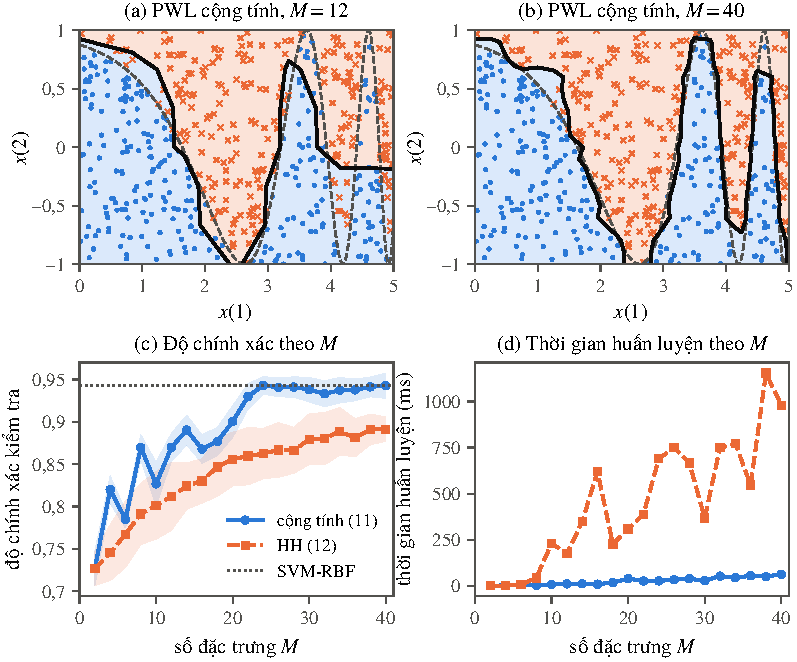
\includegraphics[width=0.78\linewidth]{fig_cosexp_M.pdf}
\caption[Tái hiện thí nghiệm Cosexp: ảnh hưởng của số đặc trưng]{Tái hiện thí nghiệm Cosexp (Hình~3 của~\cite{huang2013}), $10$ lần lặp. (a), (b) Biên của PWL-C-SVM cộng tính với $M=12$ và $M=40$ (nét liền) so với biên thật (nét đứt). (c) Độ chính xác trên tập kiểm tra theo $M$: đường là trung bình, dải màu là $\pm$ một độ lệch chuẩn; đường chấm là SVM hạt nhân Gauss. (d) Thời gian huấn luyện (trung vị) với $\gamma$ đã chọn.}
\label{fig:cosexp}
\end{figure}

Xu hướng mà bài báo gốc báo cáo được tái hiện đúng. Với $M=2$, bộ phân loại chỉ là tuyến tính và đạt $72{,}7\pm2{,}0\%$ (bài báo: $76{,}83\%$ với một lần chạy). Khi $M$ tăng, biên bám sát đường cong thật hơn; độ chính xác đạt $90{,}0\%$ tại $M=20=10n$ và ổn định quanh $94\%$ từ $M=24$, ngang SVM hạt nhân Gauss ($94{,}2\pm0{,}9\%$), trong khi thời gian huấn luyện vẫn dưới $0{,}1$ giây. Ánh xạ HH kém hẳn ($89{,}1\pm1{,}4\%$ tại $M=40$) dù về lý thuyết linh hoạt hơn, vì nhãn của Cosexp được xác định bởi một hàm cộng tính: ánh xạ cộng tính khớp đúng cấu trúc đó, còn các siêu phẳng ngẫu nhiên của HH phân tán khả năng biểu diễn vào những hướng không cần thiết. Cùng với \cref{sec:exp2d}, điều này cho một quy tắc thực hành, cũng là thứ tự mà bài báo gốc khuyến nghị~\cite[Mục~4]{huang2013}: thử ánh xạ cộng tính trước, vì nó rẻ, dễ diễn giải và đủ tốt khi tương tác giữa các biến yếu; chỉ chuyển sang HH khi có dấu hiệu tương tác mạnh.

% ----------------------------------------------------------------------------
\subsection{Mười bộ dữ liệu chuẩn}\label{sec:bench10}

\paragraph{Dữ liệu và giao thức.} Đề án dùng mười bộ dữ liệu phân loại nhị phân (\cref{tab:datasets}): bảy bộ có trong Bảng~1 của bài báo gốc và ba bộ (Banknote, Spambase, Sonar) được thêm vào để đa dạng hóa kích thước và số chiều. Mỗi bộ được chia ngẫu nhiên có phân tầng thành hai nửa huấn luyện và kiểm tra, lặp lại $10$ lần ($5$ lần với Spambase, do chi phí tinh chỉnh các mô hình hạt nhân); với Magic, tập huấn luyện gồm $2.000$ điểm như trong bài báo gốc. Tham số được chọn bằng kiểm định chéo $10$ phần trên tập huấn luyện: $\gamma\in\{2^{-5},2^{-3},\dots,2^{11}\}$ cho mọi mô hình SVM, $1/\sigma^2\in\{2^{-15},2^{-13},\dots,2^{3}\}$ cho hạt nhân Gauss theo khuyến nghị của~\cite{hsu2003}, và hệ số phạt $L_2$ trong $\{10^{-4},10^{-3},\dots,1\}$ cho mạng nơ-ron. Chín phương pháp được so sánh: SVM tuyến tính; SVM và LS-SVM hạt nhân Gauss; kNN với $k=1$ như trong bài báo; Ik-SVM; mạng nơ-ron một lớp ẩn gồm $9n$ nơ-ron ReLU --- bằng số đặc trưng bản lề của PWL-SVM dạng HH --- huấn luyện bằng L-BFGS~\cite{liu1989}; và ba biến thể PWL-SVM với $M/n=10$ theo đúng quy tắc của bài báo: PWL-C-SVM và PWL-LS-SVM với ánh xạ cộng tính lưới đều, và PWL-C-SVM với ánh xạ HH chuẩn hóa $|p(1)|=1$.

\begin{table}[t]
\centering
\caption[Mười bộ dữ liệu chuẩn]{Mười bộ dữ liệu chuẩn, sắp theo số chiều $n$ (sau khi bỏ các cột hằng). $N$ là số mẫu, cột cuối là số mẫu huấn luyện/kiểm tra trong mỗi lần chia.}
\label{tab:datasets}
\small
\renewcommand{\arraystretch}{1.15}
\setlength{\tabcolsep}{4.5pt}
\begin{tabular}{@{}l l r r r r@{}}
\toprule
\textbf{Tên} & \textbf{Nội dung} & $N$ & $n$ & \begin{tabular}[b]{@{}c@{}}\textbf{\% lớp}\\ \textbf{$+1$}\end{tabular} & \begin{tabular}[b]{@{}c@{}}\textbf{Huấn luyện/}\\ \textbf{kiểm tra}\end{tabular}\\
\midrule
Haberman & sống sót sau phẫu thuật ung thư vú & 306 & 3 & 26{,}5 & 153/153\\
Transfusion & hiến máu tình nguyện & 748 & 4 & 23{,}8 & 374/374\\
Banknote & xác thực tiền giấy & 1.372 & 4 & 44{,}5 & 686/686\\
Pima & bệnh tiểu đường & 768 & 8 & 34{,}9 & 384/384\\
Breast & ung thư vú Wisconsin (bản gốc) & 699 & 9 & 34{,}5 & 349/350\\
Magic & kính thiên văn tia gamma & 19.020 & 10 & 35{,}2 & 2.000/17.020\\
Parkinsons & bệnh Parkinson (giọng nói) & 195 & 22 & 75{,}4 & 97/98\\
Ionosphere & tín hiệu radar tầng điện li & 351 & 33 & 64{,}1 & 175/176\\
Spambase & thư rác & 4.601 & 57 & 39{,}4 & 2.300/2.301\\
Sonar & tín hiệu sonar (đá hay mìn) & 208 & 60 & 53{,}4 & 104/104\\
\bottomrule
\end{tabular}
\end{table}


\begin{table}[t]
\centering
\caption[Độ chính xác trên mười bộ dữ liệu chuẩn]{Độ chính xác trung bình trên tập kiểm tra (\%) qua $10$ lần chia ngẫu nhiên ($5$ lần với Spambase). In đậm: giá trị cao nhất mỗi hàng. Dòng cuối là hạng trung bình trên mười bộ dữ liệu ($1$ là tốt nhất). Độ lệch chuẩn được cho ở \cref{tab:appendix-bench} (Phụ lục~B).}
\label{tab:bench}
\footnotesize
\setlength{\tabcolsep}{3pt}
\renewcommand{\arraystretch}{1.18}
\resizebox{\linewidth}{!}{%
\begin{tabular}{@{}l r r r r r r r r r@{}}
\toprule
\textbf{Dữ liệu} & \begin{tabular}[b]{@{}c@{}}SVM\\tuyến tính\end{tabular} & \begin{tabular}[b]{@{}c@{}}SVM-\\RBF\end{tabular} & \begin{tabular}[b]{@{}c@{}}LS-SVM-\\RBF\end{tabular} & \begin{tabular}[b]{@{}c@{}}kNN\\$(k=1)$\end{tabular} & \begin{tabular}[b]{@{}c@{}}Ik-\\SVM\end{tabular} & \begin{tabular}[b]{@{}c@{}}MLP-\\ReLU\end{tabular} & \begin{tabular}[b]{@{}c@{}}PWL-C\\cộng tính\end{tabular} & \begin{tabular}[b]{@{}c@{}}PWL-LS\\cộng tính\end{tabular} & \begin{tabular}[b]{@{}c@{}}PWL-C\\HH\end{tabular}\\
\midrule
Haberman & 72{,}5 & 73{,}3 & 73{,}4 & 65{,}7 & 72{,}0 & 72{,}4 & 73{,}2 & 72{,}6 & \textbf{73{,}5}\\
Transfusion & 76{,}5 & 77{,}6 & 77{,}7 & 68{,}4 & 76{,}7 & \textbf{78{,}6} & 76{,}3 & 77{,}4 & 76{,}3\\
Banknote & 98{,}6 & \textbf{100{,}0} & \textbf{100{,}0} & 99{,}8 & 99{,}9 & 99{,}9 & 99{,}9 & 99{,}5 & 99{,}9\\
Pima & \textbf{76{,}7} & 76{,}1 & 76{,}6 & 70{,}8 & 76{,}0 & \textbf{76{,}7} & 76{,}3 & 76{,}5 & 76{,}2\\
Breast & 96{,}6 & 96{,}5 & 96{,}4 & 95{,}3 & 96{,}4 & \textbf{96{,}8} & 96{,}3 & 96{,}0 & 95{,}6\\
Magic & 79{,}0 & 85{,}5 & 85{,}6 & 78{,}3 & 85{,}0 & \textbf{85{,}7} & 84{,}8 & 84{,}4 & 84{,}3\\
Parkinsons & 85{,}4 & 89{,}9 & 91{,}4 & \textbf{93{,}7} & 89{,}4 & 90{,}6 & 86{,}2 & 89{,}3 & 85{,}5\\
Ionosphere & 86{,}2 & 93{,}4 & \textbf{93{,}8} & 86{,}4 & 91{,}1 & 88{,}0 & 89{,}7 & 87{,}7 & 87{,}0\\
Spambase & 93{,}0 & 93{,}6 & 93{,}4 & 88{,}8 & \textbf{94{,}6} & 93{,}9 & 93{,}4 & 92{,}6 & 82{,}1\\
Sonar & 75{,}2 & 84{,}3 & \textbf{84{,}5} & 81{,}2 & 82{,}0 & 81{,}9 & 80{,}2 & 79{,}8 & 76{,}2\\
\midrule
Hạng trung bình & 6{,}55 & 3{,}15 & 2{,}35 & 7{,}40 & 4{,}60 & 3{,}00 & 5{,}35 & 6{,}00 & 6{,}60\\
\bottomrule
\end{tabular}}
\end{table}


\begin{table}[t]
\centering
\caption[So sánh theo cặp với PWL-C-SVM cộng tính]{So sánh theo cặp giữa PWL-C-SVM cộng tính và từng phương pháp khác trên mười bộ dữ liệu: số bộ mà PWL-C-SVM cao hơn / bằng / thấp hơn và chênh lệch trung bình (tính trên các giá trị của \cref{tab:bench}), cùng giá trị $p$ của kiểm định dấu hạng Wilcoxon hai phía trên độ chính xác trung bình chưa làm tròn, chưa hiệu chỉnh cho so sánh bội.}
\label{tab:wilcoxon}
\small
\renewcommand{\arraystretch}{1.18}
\begin{tabular}{@{}l c r r@{}}
\toprule
\textbf{Phương pháp so sánh} & \textbf{Cao hơn / bằng / thấp hơn} & \textbf{Chênh lệch TB} & $p$\\
\midrule
SVM tuyến tính & 7 / 0 / 3 & $+1{,}66$ & 0{,}037\\
SVM-RBF & 1 / 0 / 9 & $-1{,}39$ & 0{,}020\\
LS-SVM-RBF & 0 / 1 / 9 & $-1{,}65$ & 0{,}002\\
kNN ($k=1$) & 8 / 0 / 2 & $+2{,}79$ & 0{,}084\\
Ik-SVM & 2 / 1 / 7 & $-0{,}68$ & 0{,}105\\
MLP-ReLU & 2 / 1 / 7 & $-0{,}82$ & 0{,}139\\
PWL-LS-SVM cộng tính & 7 / 0 / 3 & $+0{,}05$ & 0{,}432\\
PWL-C-SVM HH & 7 / 2 / 1 & $+1{,}97$ & 0{,}027\\
\bottomrule
\end{tabular}
\end{table}


\paragraph{Kết quả.} Ba phương pháp dẫn đầu về độ chính xác (\cref{tab:bench}) là LS-SVM hạt nhân Gauss, mạng nơ-ron và SVM hạt nhân Gauss, với hạng trung bình lần lượt $2{,}35$, $3{,}00$ và $3{,}15$; PWL-C-SVM cộng tính đứng giữa bảng (hạng $5{,}35$), trên SVM tuyến tính ($6{,}55$) và kNN ($7{,}40$). Trên năm bộ Haberman, Transfusion, Banknote, Pima và Breast, mọi phương pháp dựa trên SVM, kể cả SVM tuyến tính, chênh nhau không quá khoảng $1{,}5$ điểm phần trăm: một biên tuyến tính đã gần như đủ tốt. Trên bốn bộ Magic, Parkinsons, Ionosphere và Sonar, nơi SVM tuyến tính kém SVM hạt nhân Gauss từ $4$ đến $9$ điểm, PWL-C-SVM cộng tính thu hẹp đáng kể khoảng cách trên ba bộ (hơn SVM tuyến tính $5{,}8$ điểm trên Magic, $3{,}5$ điểm trên Ionosphere và $5{,}0$ điểm trên Sonar) nhưng vẫn kém SVM hạt nhân Gauss từ $0{,}7$ đến $4{,}1$ điểm. Để so sánh hai bộ phân loại trên nhiều bộ dữ liệu, Demšar~\cite{demsar2006} khuyến nghị kiểm định dấu hạng Wilcoxon; \cref{tab:wilcoxon} áp dụng kiểm định này cho PWL-C-SVM cộng tính và từng phương pháp khác. Với hai so sánh chính của câu hỏi CH1, PWL-C-SVM cộng tính kém SVM hạt nhân Gauss ($p=0{,}020$) và cao hơn SVM tuyến tính trên bảy trong mười bộ, với chênh lệch trung bình $1{,}7$ điểm ($p=0{,}037$); sau hiệu chỉnh Holm cho hai phép so sánh, cả hai khác biệt vẫn có ý nghĩa ở mức $5\%$ (giá trị $p$ hiệu chỉnh đều bằng $0{,}039$). Các giá trị $p$ khác trong \cref{tab:wilcoxon} chưa được hiệu chỉnh cho so sánh bội: nếu hiệu chỉnh Holm cho cả tám phép so sánh, chỉ khác biệt so với LS-SVM hạt nhân Gauss còn có ý nghĩa ở mức $5\%$. Với chỉ mười bộ dữ liệu, các kiểm định này có lực thấp, nên “không bác bỏ” không có nghĩa là “tương đương”.

\paragraph{So với bài báo gốc.} Kết quả trên không xác nhận nhận định của bài báo gốc rằng PWL-SVM có độ chính xác tương đương SVM hạt nhân Gauss~\cite{huang2013}. Nguyên nhân chính là bài báo chỉ dùng một lần chia dữ liệu: trên các bộ nhỏ như Parkinsons ($98$ điểm kiểm tra), độ lệch chuẩn giữa các lần chia lên tới $2$--$4$ điểm phần trăm, và bài báo báo cáo độ chính xác $100\%$ cho PWL-C-SVM trên bộ này, trong khi trung bình qua mười lần chia chỉ là $86{,}2\%$. Ngược lại, lợi thế về kích thước mô hình được xác nhận rõ ràng: với ánh xạ cộng tính, PWL-C-SVM cần từ $64$ đến $1.261$ số thực, nhỏ hơn SVM hạt nhân Gauss từ $2{,}5$ đến $36$ lần (Phụ lục~B). Trường hợp đáng chú ý nhất là Magic: PWL-C-SVM đạt $84{,}8\%$ so với $85{,}5\%$ của SVM hạt nhân Gauss với một mô hình gồm $211$ số thực thay vì $7.694$.

\paragraph{Ánh xạ HH.} PWL-C-SVM với ánh xạ HH có hạng trung bình thấp ($6{,}60$), chủ yếu do quy tắc sinh tham số chứ không phải do mô hình. Trên Spambase, ở lần chia đầu tiên, mô hình thất bại hoàn toàn ($40{,}0\%$, thấp hơn cả tỉ lệ $60{,}6\%$ của lớp đa số), trong khi ở bốn lần chia còn lại nó đạt từ $91{,}0\%$ đến $93{,}7\%$. Nguyên nhân là dữ liệu này rất thưa (gần $78\%$ giá trị bằng $0$ sau khi chuẩn hóa), nên nhiều siêu phẳng đi qua các điểm lấy đều trong hình hộp $[0,1]^{57}$ không cắt qua vùng dữ liệu, còn quy tắc $|p(1)|=1$ (\cref{rem:scale}) làm giá trị lớn nhất của các đặc trưng trên tập huấn luyện dao động từ $423$ đến $3{,}3\cdot10^{5}$ giữa các lần chia, khiến bài toán tối ưu bị điều kiện hóa rất kém. Chỉ cần chuẩn hóa $\|p\|_2=1$, PWL-C-SVM HH đạt $93{,}4\pm0{,}2\%$ trên Spambase. Ngoài ra, mạng nơ-ron với cùng số nơ-ron ẩn tốt hơn PWL-C-SVM HH trên tám trong mười bộ: học lớp ẩn từ dữ liệu có lợi hơn nhiều so với sinh nó ngẫu nhiên, và đó là cái giá của tính lồi đã nêu ở Mục~\ref{sec:pwlsvm}.

% ----------------------------------------------------------------------------
\subsection{Ảnh hưởng của số đặc trưng và của quy tắc chọn tham số}\label{sec:sensitivity}

Để trả lời câu hỏi CH3 một cách có kiểm soát, ta cố định mô hình là PWL-LS-SVM, giải chính xác bằng hồi quy ridge (\cref{prop:ridge}) để loại trừ ảnh hưởng của bộ giải, và thay đổi hai yếu tố: số đặc trưng trên mỗi chiều $M/n\in\{1,2,3,5,10,20\}$ và quy tắc chọn tham số --- ánh xạ cộng tính với lưới đều (quy tắc của bài báo gốc) hoặc lưới phân vị (\cref{rem:quantile}), ánh xạ HH với $|p(1)|=1$ (quy tắc của bài báo gốc) hoặc $\|p\|_2=1$ (\cref{rem:scale}). Thí nghiệm dùng ba bộ dữ liệu có đặc điểm khác nhau --- Ionosphere ($n=33$), Magic ($n=10$, nhiều dữ liệu) và Spambase ($n=57$, rất thưa) --- với $5$ lần chia như ở Mục~\ref{sec:bench10} và $\gamma$ chọn bằng kiểm định chéo $5$ phần (\cref{fig:sensitivity}).

\begin{figure}[t]
\centering
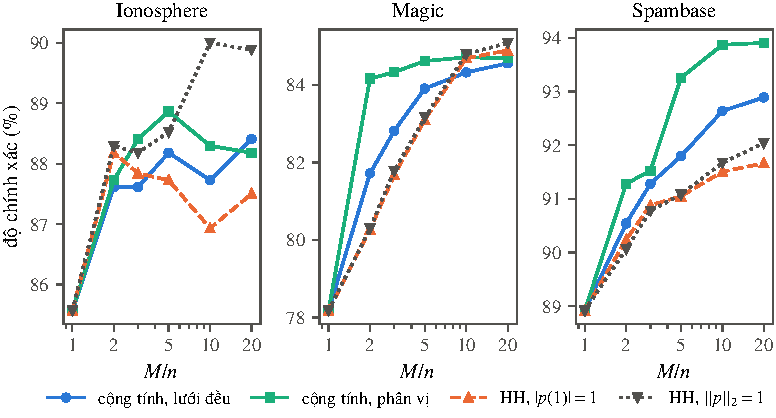
\includegraphics[width=0.84\linewidth]{fig_sensitivity.pdf}
\caption[Ảnh hưởng của số đặc trưng và quy tắc chọn tham số]{Độ chính xác trung bình (qua $5$ lần chia) của PWL-LS-SVM theo số đặc trưng trên mỗi chiều $M/n$, với bốn quy tắc chọn tham số. $M/n=1$ ứng với bộ phân loại tuyến tính.}
\label{fig:sensitivity}
\end{figure}

Có ba nhận xét. Thứ nhất, độ chính xác tăng nhanh khi $M/n$ tăng từ $1$ và bão hòa quanh $M/n=5$--$10$, phù hợp với quy tắc $M=10n$ của bài báo gốc. Thứ hai, lưới phân vị tốt hơn hoặc ngang lưới đều trên cả ba bộ, rõ nhất khi phân bố lệch: trên Magic, nó đạt $84{,}2\%$ ngay với $M/n=2$, trong khi lưới đều cần $M/n=10$ để đạt $84{,}3\%$; trên Spambase, nó đạt $93{,}9\%$ so với $92{,}6\%$ của lưới đều ở $M/n=10$ mà chỉ dùng $156$ thay vì $570$ đặc trưng, vì các nút trùng nhau bị loại bỏ. Thứ ba, ánh xạ HH cần nhiều đặc trưng hơn hẳn mới đuổi kịp ánh xạ cộng tính: trên Magic, nó chỉ ngang lưới phân vị khi $M/n\ge10$ (nhỉnh hơn $0{,}4$ điểm ở $M/n=20$), trên Spambase nó kém ở mọi giá trị của $M/n$; chỉ trên Ionosphere, nơi tương tác giữa các biến có vai trò, HH với $\|p\|_2=1$ tốt nhất rõ rệt ($90{,}0\%$ ở $M/n=10$, so với $86{,}9\%$ với $|p(1)|=1$). Chuẩn hóa $\|p\|_2=1$ không làm kết quả xấu đi đáng kể ở bất kỳ cấu hình nào. Từ đó rút ra quy trình được dùng cho dữ liệu dạng bảng ở phần còn lại của chương: ánh xạ cộng tính, nút theo phân vị, $M/n$ từ $5$ đến $10$; chỉ dùng ánh xạ HH, với các siêu phẳng được chuẩn hóa, khi có dấu hiệu tương tác mạnh giữa các biến.


\section{Chi phí tính toán và bộ nhớ}\label{sec:cost}

Mục~\ref{sec:pwlsvm} dự báo rằng lợi thế của PWL-SVM nằm ở khâu dự đoán, vốn chỉ gồm các phép so sánh, nhân, cộng và lấy cực đại (\cref{tab:cost}). Dự báo này được kiểm tra trên Magic ($9.510$ mẫu huấn luyện, chia đôi toàn bộ dữ liệu) và dữ liệu tín dụng của Mục~\ref{sec:application} ($21.000$ mẫu huấn luyện). Mọi mô hình chạy trên một luồng xử lý của cùng một máy tính, khi không có tiến trình nặng nào khác; tham số được chọn trước bằng kiểm định chéo trên một mẫu con $4.000$ điểm, và chỉ thời gian của một lần huấn luyện với tham số đã chọn được đo; thời gian dự đoán là trung vị của bảy lần dự đoán toàn bộ tập kiểm tra, chia cho số mẫu. PWL-SVM dùng ánh xạ cộng tính với nút phân vị và $M/n=10$ (Mục~\ref{sec:sensitivity}). Kết quả được cho ở \cref{tab:cost-measured}.

\begin{table}[t]
\centering
\caption[Chi phí huấn luyện, dự đoán và bộ nhớ]{Chi phí trên Magic ($9.510$ mẫu huấn luyện) và dữ liệu tín dụng ($21.000$ mẫu huấn luyện), đo trên một luồng xử lý: thời gian huấn luyện một mô hình với tham số đã chọn, thời gian dự đoán mỗi mẫu, số thực cần lưu, và độ chính xác (Magic) hoặc AUC (tín dụng) trên tập kiểm tra. Đây là một lần chia riêng, với tham số chọn trên mẫu con (và với Magic, tập huấn luyện lớn hơn nhiều), nên độ chính xác khác với ở \cref{tab:bench,tab:credit}.}
\label{tab:cost-measured}
\footnotesize
\setlength{\tabcolsep}{3pt}
\renewcommand{\arraystretch}{1.18}
\begin{tabular}{@{}l r r r c r r r c@{}}
\toprule
 & \multicolumn{4}{c}{\textbf{Magic}} & \multicolumn{4}{c}{\textbf{Tín dụng}}\\
\cmidrule(lr){2-5}\cmidrule(l){6-9}
\textbf{Mô hình} & \begin{tabular}[b]{@{}c@{}}\textbf{Huấn}\\\textbf{luyện (s)}\end{tabular} & \begin{tabular}[b]{@{}c@{}}\textbf{Dự đoán}\\\textbf{($\mu$s/mẫu)}\end{tabular} & \begin{tabular}[b]{@{}c@{}}\textbf{Số}\\\textbf{thực}\end{tabular} & \begin{tabular}[b]{@{}c@{}}\textbf{ĐCX}\\\textbf{(\%)}\end{tabular} & \begin{tabular}[b]{@{}c@{}}\textbf{Huấn}\\\textbf{luyện (s)}\end{tabular} & \begin{tabular}[b]{@{}c@{}}\textbf{Dự đoán}\\\textbf{($\mu$s/mẫu)}\end{tabular} & \begin{tabular}[b]{@{}c@{}}\textbf{Số}\\\textbf{thực}\end{tabular} & \textbf{AUC}\\
\midrule
SVM tuyến tính & 5{,}2 & 0{,}02 & 31 & 78{,}7 & 9{,}3 & 0{,}06 & 79 & 0{,}694\\
Hồi quy logistic & 0{,}00 & 0{,}02 & 31 & 78{,}7 & 0{,}02 & 0{,}05 & 79 & 0{,}716\\
Thẻ điểm & 0{,}02 & 0{,}69 & 191 & 84{,}6 & 0{,}07 & 1{,}4 & 379 & 0{,}768\\
PWL-C-SVM, cộng tính & 4{,}7 & 0{,}33 & 211 & 85{,}7 & 52 & 0{,}58 & 349 & 0{,}685\\
PWL-LS-SVM, cộng tính & 0{,}01 & 0{,}33 & 211 & 84{,}8 & 0{,}04 & 0{,}56 & 349 & 0{,}768\\
PWL-LS-SVM, HH & 0{,}01 & 0{,}40 & 1.111 & 85{,}1 & 0{,}07 & 1{,}3 & 6.631 & 0{,}740\\
SVM-RBF & 0{,}76 & 64{,}7 & 34.462 & 87{,}1 & 4{,}6 & 241 & 239.111 & 0{,}711\\
MLP-ReLU & 2{,}9 & 0{,}18 & 1.101 & 86{,}5 & 21 & 0{,}57 & 6.605 & 0{,}761\\
Tổ hợp cây tăng cường & 0{,}11 & 3{,}8 & 12.200 & 88{,}1 & 0{,}15 & 1{,}4 & 4.514 & 0{,}774\\
\bottomrule
\end{tabular}
\end{table}


PWL-LS-SVM cộng tính dự đoán mỗi mẫu trong $0{,}33$~$\mu$s trên Magic và $0{,}56$~$\mu$s trên dữ liệu tín dụng, nhanh hơn SVM hạt nhân Gauss khoảng 200 và 430 lần. Chênh lệch đến từ cấu trúc của mô hình: trên dữ liệu tín dụng, SVM hạt nhân Gauss lưu $239.111$ số thực, ứng với khoảng $8.854$ vectơ hỗ trợ, và mỗi lần dự đoán phải tính chừng ấy khoảng cách cùng hàm mũ, còn PWL-SVM cộng tính chỉ lưu $349$ số và thực hiện vài trăm phép so sánh, nhân và cộng, đúng như các công thức ở \cref{tab:cost}. Trên dữ liệu tín dụng, mạng nơ-ron dự đoán nhanh ngang PWL-SVM cộng tính nhưng lớn hơn khoảng 19 lần; tổ hợp cây tăng cường và thẻ điểm (có kích thước tương đương PWL-SVM) dự đoán chậm hơn khoảng 2{,}5 và 2{,}6 lần. Chỉ các mô hình tuyến tính trên biến gốc là nhỏ và nhanh hơn PWL-SVM, với cái giá là độ chính xác thấp hơn rõ rệt: trên Magic, hồi quy logistic đạt $78{,}7\%$ so với $84{,}8\%$ của PWL-LS-SVM cộng tính.

Về huấn luyện, PWL-LS-SVM là mô hình phi tuyến huấn luyện nhanh nhất ($0{,}01$ giây trên Magic và $0{,}04$ giây trên dữ liệu tín dụng), vì chỉ cần lập và giải một hệ tuyến tính cỡ $M\times M$ (\cref{prop:ridge}). PWL-C-SVM chậm hơn nhiều ($4{,}7$ và $52$ giây) do bộ giải lặp của LIBLINEAR; SVM hạt nhân Gauss cần $0{,}76$ và $4{,}6$ giây, và chi phí này tăng nhanh hơn tuyến tính theo số mẫu~\cite{chang2011}. Các số đo tuyệt đối phụ thuộc vào cài đặt --- PWL-SVM được cài bằng NumPy, còn LIBSVM là thư viện C đã được tối ưu nhiều năm; trên một thiết bị nhúng, số phép tính và số thực cần lưu ở \cref{tab:cost} mới là thước đo phù hợp, và ở cả hai thước đo đó PWL-SVM cộng tính có lợi thế lớn so với SVM hạt nhân Gauss.

% ----------------------------------------------------------------------------
\section{Ứng dụng: dự báo vỡ nợ thẻ tín dụng}\label{sec:application}

\subsection{Bài toán và dữ liệu}

Ngân hàng phát hành thẻ tín dụng cần ước lượng khả năng một khách hàng không thanh toán được dư nợ trong kỳ tới để điều chỉnh hạn mức, ưu tiên nhắc nợ hoặc trích lập dự phòng rủi ro. Đây là một bài toán phân loại nhị phân điển hình của chấm điểm tín dụng~\cite{thomas2002}, và cả ba yêu cầu nêu ở Mở đầu đều có mặt: độ chính xác quyết định trực tiếp chi phí rủi ro; số hồ sơ lớn và được chấm điểm định kỳ; và quyết định phải giải thích được với khách hàng cũng như với cơ quan quản lý.

Đề án dùng dữ liệu của Yeh và Lien~\cite{yeh2009} về $30.000$ chủ thẻ tín dụng của một ngân hàng ở Đài Loan, từ tháng 4 đến tháng 9 năm 2005. Nhãn cho biết khách hàng có vỡ nợ trong tháng tiếp theo hay không; có $6.636$ khách hàng vỡ nợ, tức $22{,}1\%$. Hai mươi ba biến giải thích gồm hạn mức tín dụng (LIMIT\_BAL), bốn biến nhân khẩu học (SEX, EDUCATION, MARRIAGE, AGE), trạng thái trả nợ của sáu tháng gần nhất (PAY\_0, PAY\_2, \dots, PAY\_6) cùng các số tiền sao kê (BILL\_AMT1--6) và đã thanh toán (PAY\_AMT1--6) tương ứng; ý nghĩa và cách mã hóa từng biến được cho ở \cref{tab:credit-vars} (Phụ lục~C). Sau khi mã hóa các biến định danh, mỗi khách hàng được mô tả bởi $n=26$ đặc trưng số.

Hai đặc điểm của dữ liệu quyết định thiết kế mô hình (\cref{fig:credit-overview}). Thứ nhất, quan hệ giữa lịch sử trả nợ và rủi ro là phi tuyến rõ rệt: tỉ lệ vỡ nợ gần như không đổi, khoảng $13$--$17\%$, với các trạng thái $-2$, $-1$ và $0$, rồi tăng vọt lên $34\%$ khi chậm một tháng và gần $70\%$ khi chậm hai tháng --- một bước nhảy mà mô hình tuyến tính theo PAY\_0 không mô tả được, nhưng một hàm tuyến tính từng phần với vài điểm gãy thì có thể. Thứ hai, các biến tiền tệ lệch rất mạnh: hạn mức trải từ $10$ nghìn đến $1$ triệu Đài tệ, nhưng một nửa số khách hàng có hạn mức không vượt quá $140$ nghìn. Lưới nút đều của bài báo gốc vì vậy đặt phần lớn các nút ở vùng gần như không có dữ liệu, còn lưới theo phân vị (\cref{rem:quantile}) đặt nút theo mật độ dữ liệu.

\begin{figure}[t]
\centering
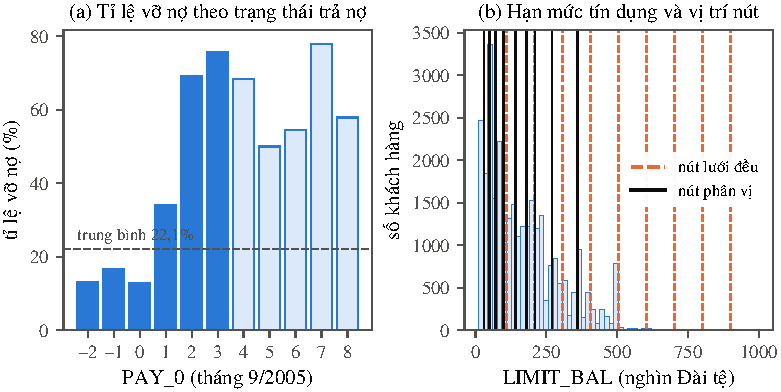
\includegraphics[width=0.84\linewidth]{fig_credit_overview.pdf}
\caption[Hai đặc điểm của dữ liệu tín dụng]{(a) Tỉ lệ vỡ nợ theo trạng thái trả nợ tháng 9 (PAY\_0); cột nhạt ứng với các nhóm có ít hơn $100$ khách hàng. (b) Phân bố hạn mức tín dụng cùng vị trí $9$ nút của lưới đều (nét đứt) và của lưới theo phân vị (nét liền).}
\label{fig:credit-overview}
\end{figure}

\subsection{Thiết kế thực nghiệm}

Dữ liệu được chia ngẫu nhiên có phân tầng theo tỉ lệ $70/30$, thành $21.000$ khách hàng huấn luyện và $9.000$ khách hàng kiểm tra, lặp lại $5$ lần. Độ đo chính là diện tích dưới đường cong ROC (AUC)~\cite{fawcett2006}, tức xác suất để một khách hàng vỡ nợ chọn ngẫu nhiên bị mô hình chấm điểm rủi ro cao hơn một khách hàng không vỡ nợ chọn ngẫu nhiên; AUC không phụ thuộc vào ngưỡng quyết định và được dùng phổ biến trong chấm điểm tín dụng~\cite{lessmann2015}. Ngoài ra, với ngưỡng chọn trên tập huấn luyện sao cho tỉ lệ khách hàng bị dự báo vỡ nợ bằng tỉ lệ vỡ nợ quan sát được, đề án tính độ chính xác cân bằng (trung bình của độ nhạy và độ đặc hiệu) và độ đo F1 của lớp vỡ nợ trên tập kiểm tra.

Mười mô hình được so sánh. Ba mô hình tuyến tính đóng vai trò chuẩn so sánh của ngành: hồi quy logistic trên các biến gốc, SVM tuyến tính, và \emph{thẻ điểm} --- hồi quy logistic trên các biến đã được rời rạc hóa theo cách xây dựng thẻ điểm truyền thống~\cite{thomas2002}, trong đó mỗi biến liên tục được chia thành mười khoảng theo thập phân vị và mỗi giá trị của các biến PAY là một hạng mục riêng. Bốn biến thể PWL-SVM, đều với $M/n=10$, gồm PWL-LS-SVM cộng tính với lưới đều (quy tắc của bài báo gốc) và với lưới phân vị, PWL-C-SVM cộng tính với lưới phân vị, và PWL-LS-SVM với ánh xạ HH. Ba mô hình phi tuyến làm đối chứng: SVM hạt nhân Gauss; mạng nơ-ron một lớp ẩn với $9n=234$ nơ-ron ReLU, huấn luyện bằng L-BFGS~\cite{liu1989}; và tổ hợp cây tăng cường theo gradient~\cite{friedman2001} với thiết lập mặc định của scikit-learn (có dừng sớm), đại diện cho các mô hình tổ hợp --- nhóm phương pháp cho kết quả tốt nhất trong nghiên cứu so sánh của Lessmann và cộng sự~\cite{lessmann2015}. Tham số được chọn bằng kiểm định chéo $5$ phần trên tập huấn luyện với tiêu chí AUC, trên các lưới cho ở Phụ lục~C; riêng SVM hạt nhân Gauss và mạng nơ-ron, vì chi phí huấn luyện lớn, được tinh chỉnh bằng kiểm định chéo $3$ phần trên mẫu con phân tầng gồm $5.000$ và $7.000$ khách hàng, rồi huấn luyện lại trên toàn bộ tập huấn luyện.


\subsection{Kết quả}\label{sec:credit-results}

\begin{table}[t]
\centering
\caption[Kết quả trên dữ liệu vỡ nợ thẻ tín dụng]{Kết quả trên dữ liệu vỡ nợ thẻ tín dụng (trung bình $\pm$ độ lệch chuẩn qua $5$ lần chia $70/30$). AUC: diện tích dưới đường ROC; ĐCX-CB: độ chính xác cân bằng; F1 tính cho lớp vỡ nợ; ngưỡng được chọn trên tập huấn luyện sao cho tỉ lệ dự báo vỡ nợ bằng tỉ lệ vỡ nợ quan sát. Cột cuối: số thực cần lưu (trung vị); thời gian dự đoán được đo riêng ở \cref{sec:cost}.}
\label{tab:credit}
\footnotesize
\setlength{\tabcolsep}{3pt}
\renewcommand{\arraystretch}{1.18}
\begin{tabular}{@{}l c c c r@{}}
\toprule
\textbf{Mô hình} & \textbf{AUC} & \textbf{ĐCX-CB (\%)} & \textbf{F1 (\%)} & \textbf{Số thực}\\
\midrule
Hồi quy logistic & $0{,}724\pm0{,}009$ & $68{,}7\pm0{,}6$ & $51{,}2\pm0{,}9$ & 79\\
Thẻ điểm (logistic, biến rời rạc hóa) & $0{,}773\pm0{,}006$ & $70{,}3\pm0{,}6$ & $53{,}7\pm1{,}0$ & 381\\
SVM tuyến tính & $0{,}706\pm0{,}008$ & $68{,}5\pm0{,}8$ & $50{,}9\pm1{,}4$ & 79\\
\midrule
PWL-LS-SVM, cộng tính, lưới đều & $0{,}772\pm0{,}006$ & $70{,}3\pm0{,}5$ & $53{,}6\pm0{,}9$ & 547\\
PWL-LS-SVM, cộng tính, phân vị & $0{,}776\pm0{,}006$ & $70{,}4\pm0{,}7$ & $53{,}8\pm1{,}1$ & 349\\
\quad và ràng buộc đơn điệu (Mục~\ref{sec:monotone}) & $0{,}775\pm0{,}006$ & $70{,}3\pm0{,}8$ & $53{,}7\pm1{,}2$ & 349\\
PWL-C-SVM, cộng tính, phân vị & $0{,}744\pm0{,}007$ & $67{,}8\pm0{,}8$ & $49{,}9\pm1{,}4$ & 349\\
PWL-LS-SVM, HH & $0{,}743\pm0{,}007$ & $69{,}5\pm0{,}6$ & $52{,}4\pm1{,}0$ & 6.631\\
\midrule
SVM-RBF & $0{,}716\pm0{,}010$ & $69{,}2\pm0{,}6$ & $52{,}0\pm1{,}0$ & 243.134\\
MLP-ReLU & $0{,}768\pm0{,}005$ & $70{,}0\pm0{,}4$ & $53{,}3\pm0{,}7$ & 6.605\\
Tổ hợp cây tăng cường & $0{,}779\pm0{,}006$ & $70{,}3\pm0{,}7$ & $53{,}7\pm1{,}1$ & 4.636\\
\bottomrule
\end{tabular}
\end{table}


\Cref{tab:credit} cho thấy các mô hình chia thành hai nhóm rõ rệt. Nhóm dẫn đầu gồm tổ hợp cây tăng cường (AUC trung bình 0{,}779), PWL-LS-SVM cộng tính với nút phân vị (0{,}776), thẻ điểm logistic trên các biến đã rời rạc hóa (0{,}773) và PWL-LS-SVM cộng tính với lưới đều (0{,}772); nhóm còn lại gồm hồi quy logistic trên các biến gốc (0{,}724), SVM tuyến tính (0{,}706) và SVM hạt nhân Gauss (0{,}716), còn mạng nơ-ron (0{,}768) đứng giữa hai nhóm. Độ chính xác cân bằng và độ đo F1 ở ngưỡng đã chọn dẫn tới cùng kết luận, và kết quả ổn định giữa các lần chia (độ lệch chuẩn của AUC khoảng 0{,}006).

Khoảng cách 0{,}052 đơn vị AUC giữa PWL-LS-SVM và hồi quy logistic trên các biến gốc chủ yếu đến từ quan hệ phi tuyến giữa trạng thái trả nợ và rủi ro (\cref{fig:credit-overview}a). Đối chứng công bằng nhất cho PWL-SVM cộng tính là thẻ điểm: cả hai đều là mô hình cộng tính dựa trên các khoảng của từng biến, chỉ khác ở chỗ đóng góp của mỗi biến là hàm bậc thang trong thẻ điểm và là đường gấp khúc liên tục trong PWL-SVM. PWL-LS-SVM cao hơn thẻ điểm ở bốn trong năm lần chia, nhưng chênh lệch trung bình chỉ là 0{,}002 đơn vị AUC, với kích thước mô hình tương đương (349 và 381 số thực).

Ba quan sát khác củng cố các kết luận ở \cref{sec:benchmark}. Lưới phân vị tốt hơn lưới đều (0{,}776 so với 0{,}772) với mô hình nhỏ hơn (349 so với 547 số thực). Với cùng ánh xạ, PWL-C-SVM cho AUC thấp hơn hẳn PWL-LS-SVM (0{,}744): mất mát bản lề chỉ quan tâm đến các điểm nằm gần hoặc vi phạm lề, nên giá trị hàm quyết định ở xa biên ít mang thông tin về mức độ rủi ro, còn mất mát bình phương của LS-SVM, tương đương hồi quy trên nhãn $\pm1$ (\cref{prop:ridge}), buộc điểm số của mọi khách hàng phản ánh nhãn của họ và vì thế cho thứ hạng tốt hơn; SVM hạt nhân Gauss, cũng dùng mất mát bản lề, gặp cùng hạn chế. Cuối cùng, ánh xạ HH (0{,}743) kém ánh xạ cộng tính, vì trên dữ liệu này ảnh hưởng riêng của từng biến quan trọng hơn tương tác giữa các biến.

\subsection{Diễn giải mô hình}\label{sec:credit-interp}

Vì ánh xạ là cộng tính, hàm quyết định của PWL-LS-SVM tách thành tổng các đóng góp của từng biến,
\begin{equation}\label{eq:additive-decomp}
f(x)=w_0+\sum_{i=1}^{n}h_i\bigl(x(i)\bigr),
\end{equation}
trong đó mỗi $h_i$ là một hàm tuyến tính từng phần một biến, có không quá chín điểm gãy đặt tại các phân vị của biến đó (\cref{prop:1d}). Mỗi $h_i$ đọc được trực tiếp như một thẻ điểm, trong đó số điểm cộng thêm cho mỗi khách hàng là một đường gấp khúc theo giá trị của biến. \Cref{fig:credit-shapes} vẽ sáu hàm $h_i$ có ảnh hưởng lớn nhất, sau khi trừ đi giá trị trung bình trên tập huấn luyện; giá trị dương nghĩa là rủi ro cao hơn một khách hàng trung bình.

\begin{figure}[t]
\centering
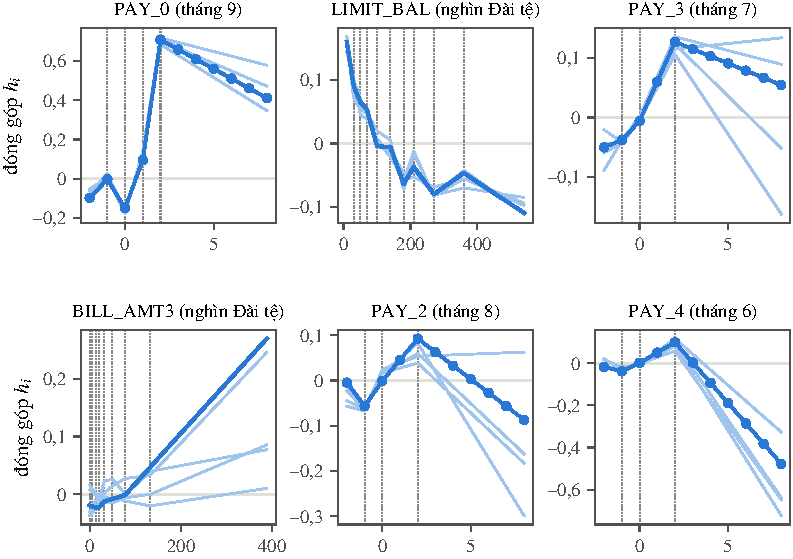
\includegraphics[width=0.82\linewidth]{fig_credit_shapes.pdf}
\caption[Các hàm đóng góp của mô hình PWL-SVM cộng tính]{Sáu hàm đóng góp $h_i$ có ảnh hưởng lớn nhất của PWL-LS-SVM cộng tính (nút phân vị) trên dữ liệu tín dụng, đã trừ giá trị trung bình. Nét đậm: mô hình của lần chia đầu tiên, nét chấm dọc là vị trí các nút của nó; nét mảnh: mô hình của bốn lần chia còn lại. Giá trị dương ứng với rủi ro vỡ nợ cao hơn.}
\label{fig:credit-shapes}
\end{figure}

Hàm đóng góp của PAY\_0 tái hiện đúng cấu trúc mà hồi quy logistic trên biến gốc bỏ lỡ (so sánh với \cref{fig:credit-overview}a): ba mã không chậm trả ($-2$, $-1$ và $0$) có đóng góp thấp và gần nhau, đóng góp tăng mạnh khi khách hàng chậm trả một tháng (tỉ lệ vỡ nợ 33{,}9\%) và đạt cực đại khi chậm hai tháng (69{,}1\%); chênh lệch giữa mã $0$ và mã $2$ là $0{,}86$ đơn vị điểm, lớn hơn toàn bộ biên độ của bất kỳ biến nào khác. Đóng góp của hạn mức tín dụng giảm dần theo hạn mức --- điều hợp lý, vì hạn mức do chính ngân hàng xác định dựa trên đánh giá tín nhiệm --- và khoảng 60\% mức giảm diễn ra ở vùng hạn mức dưới $100$ nghìn Đài tệ; trạng thái trả nợ của các tháng trước có hình dạng tương tự PAY\_0 nhưng biên độ nhỏ hơn nhiều. Ở vùng có nhiều dữ liệu, các hàm này gần như không đổi giữa các lần chia (nét mảnh ở \cref{fig:credit-shapes}): giữa phân vị $5\%$ và $95\%$ của hạn mức, đóng góp của LIMIT\_BAL ở bốn lần chia còn lại lệch khỏi lần chia đầu tiên không quá 15\% biên độ của nó, và ở các trạng thái từ $-2$ đến $2$, đóng góp của PAY\_0 lệch không quá 10\% biên độ. Thứ hạng của các biến, đo bằng độ lệch chuẩn của đóng góp $h_i$ trên tập huấn luyện, cũng ổn định: ở cả năm lần chia, PAY\_0 là biến có ảnh hưởng lớn nhất và LIMIT\_BAL đứng thứ hai; thứ tự của các biến tiếp theo, vốn có mức ảnh hưởng gần nhau, thì thay đổi giữa các lần chia; các biến nhân khẩu học (học vấn, hôn nhân, giới tính, tuổi) có ảnh hưởng nhỏ.

Hai đặc điểm khác cần được đọc thận trọng. Thứ nhất, sau mức chậm hai tháng, đóng góp của PAY\_0 và nhất là của PAY\_4 lại giảm, trái với trực giác. Đây là hệ quả của việc có quá ít dữ liệu chứ không phải quy luật thật: chỉ 1{,}5\% khách hàng có PAY\_0 từ $3$ trở lên, tỉ lệ vỡ nợ của nhóm này (71{,}9\%) không thấp hơn của nhóm chậm hai tháng, và các lần chia cho những đường rất khác nhau ở vùng này (độ lệch chuẩn giữa các lần chia lớn gấp khoảng 8 lần so với ở các trạng thái từ $-2$ đến $2$); Mục~\ref{sec:monotone} sẽ khắc phục hiện tượng này. Thứ hai, các biến dư nợ sao kê BILL\_AMT1--6 tương quan rất mạnh với nhau (hệ số tương quan giữa hai tháng liền kề từ $0{,}92$ đến $0{,}95$), nên mô hình có thể chuyển ảnh hưởng qua lại giữa chúng --- đóng góp của BILL\_AMT3 tăng theo dư nợ, còn của BILL\_AMT4 lại giảm --- và chỉ tổng đóng góp của cả nhóm mới nên được diễn giải. Đây là hạn chế chung của mọi mô hình cộng tính khi các biến tương quan mạnh, không riêng gì PWL-SVM.

Vì hàm quyết định~\eqref{eq:additive-decomp} là một tổng, mỗi quyết định của mô hình được giải thích một cách chính xác chứ không phải xấp xỉ: điểm của một khách hàng bằng điểm trung bình trên tập huấn luyện cộng với tổng các đóng góp của từng biến so với khách hàng trung bình. Chẳng hạn, khách hàng có điểm rủi ro cao nhất trong số những người vỡ nợ ở tập kiểm tra có điểm $0{,}96$, so với điểm trung bình $-0{,}56$ và ngưỡng phân loại $-0{,}44$; trong phần chênh lệch $1{,}51$, việc chậm trả hai tháng ở tháng 9 đóng góp $0{,}71$, lịch sử chậm trả ở năm tháng trước đó đóng góp thêm $0{,}63$, và hạn mức thấp ($20.000$ Đài tệ) đóng góp $0{,}13$. Một lời giải thích như vậy có thể được trình bày trực tiếp cho cán bộ tín dụng hay cho khách hàng; với SVM hạt nhân Gauss hay tổ hợp cây, nó đòi hỏi những kỹ thuật bổ sung được tính sau khi huấn luyện, chẳng hạn giá trị SHAP~\cite{lundberg2017}.

\subsection{Ràng buộc đơn điệu}\label{sec:monotone}

Người làm tín dụng kỳ vọng rằng rủi ro không giảm khi số tháng chậm trả tăng và không tăng khi hạn mức tín dụng tăng. Mô hình không ràng buộc vi phạm kỳ vọng này ở chính những đoạn được ước lượng từ rất ít dữ liệu: ở cả năm lần chia, ít nhất một trong sáu hàm $h_i$ của các biến PAY có đoạn với hệ số góc âm từ trạng thái $0$ trở đi, và hàm của LIMIT\_BAL có đoạn đi lên ở cả năm lần chia. Một mô hình trái với tri thức nghiệp vụ khó được chấp nhận khi thẩm định, dù độ chính xác của nó cao; vì vậy ta đưa kỳ vọng đơn điệu vào chính bài toán huấn luyện.

Với PWL-SVM cộng tính, điều này có thể làm mà vẫn giữ tính lồi. Gọi $t_{i1}<\dots<t_{iK}$ là các nút của biến thứ $i$ và $s_{i0},\dots,s_{iK}$ là hệ số góc của $h_i$ trên $K+1$ đoạn mà các nút chia ra. Khi đó
\begin{equation}\label{eq:slope-param}
h_i(t)=\sum_{j=0}^{K}s_{ij}\,G_{ij}(t),\qquad
G_{ij}(t)=\min\bigl\{(t-t_{ij})_+,\ t_{i,j+1}-t_{ij}\bigr\},
\end{equation}
với quy ước $t_{i0}=-\infty$, $t_{i,K+1}=+\infty$ (tức $G_{i0}(t)=\min\{t,t_{i1}\}$ và $G_{iK}(t)=(t-t_{iK})_+$): $G_{ij}(t)$ là độ dài phần đoạn thứ $j$ nằm bên trái $t$. Theo \cref{prop:1d}, hệ số của $x(i)$ trong ánh xạ~\eqref{eq:feature-map} bằng $s_{i0}$ và hệ số của $\bigl(x(i)-t_{ij}\bigr)_+$ bằng $s_{ij}-s_{i,j-1}$, nên~\eqref{eq:slope-param} chỉ là một cách tham số hóa khác của cùng một mô hình, và bài toán~\eqref{eq:ridge} trở thành
\[
\min_{s,\,w_0}\ \frac12\sum_{i=1}^{n}\Bigl[s_{i0}^2+\sum_{j=1}^{K}\bigl(s_{ij}-s_{i,j-1}\bigr)^2\Bigr]+\frac\gamma2\sum_{k=1}^{N}\Bigl(y_k-w_0-\sum_{i=1}^{n}h_i\bigl(x_k(i)\bigr)\Bigr)^2 .
\]
Hàm $h_i$ không giảm khi và chỉ khi $s_{ij}\ge0$ với mọi $j$, và không tăng khi và chỉ khi $s_{ij}\le0$ với mọi $j$; muốn $h_i$ đơn điệu chỉ trên một phần của trục, ta chỉ cần áp các bất đẳng thức đó cho những đoạn nằm trong phần ấy. Thêm các ràng buộc này, ta được một bài toán bình phương tối thiểu với ràng buộc cận trên các biến --- một bài toán lồi, giải được chính xác bằng thuật toán BVLS~\cite{stark1995} có sẵn trong SciPy~\cite{virtanen2020}. Khi không có ràng buộc nào, lời giải trùng với lời giải của \cref{prop:ridge} (sai khác dưới $10^{-9}$), điều được dùng để kiểm tra cài đặt.

\begin{figure}[t]
\centering
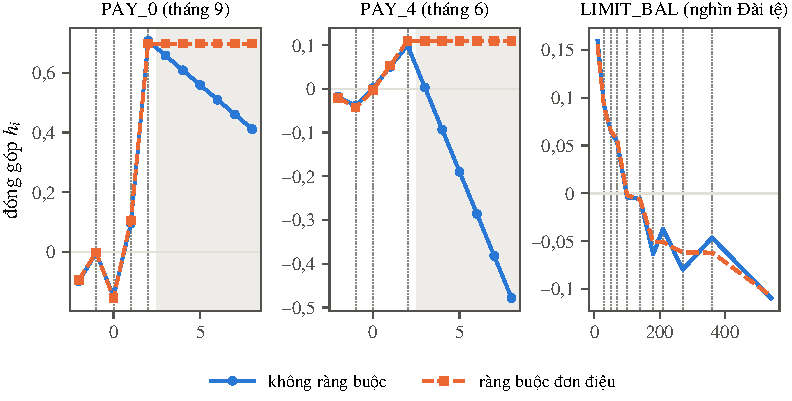
\includegraphics[width=0.84\linewidth]{fig_credit_monotone.pdf}
\caption[Hàm đóng góp khi có và không có ràng buộc đơn điệu]{Hàm đóng góp của PAY\_0, PAY\_4 và LIMIT\_BAL trong mô hình không ràng buộc (nét liền) và mô hình có ràng buộc đơn điệu (nét đứt), lần chia đầu tiên. Vùng tô xám: các trạng thái chậm trả từ ba tháng trở lên, chỉ chiếm chưa tới 2\% số khách hàng.}
\label{fig:credit-monotone}
\end{figure}

Ta ràng buộc sáu hàm của các biến PAY không giảm từ trạng thái $0$ trở đi --- ba mã $-2$, $-1$ và $0$ chỉ những tình trạng không chậm trả khác nhau, không có thứ tự tự nhiên, nên được để tự do --- và hàm của LIMIT\_BAL không tăng trên toàn miền, giữ nguyên các biến khác, các nút và hằng số $\gamma$ của mô hình không ràng buộc. \Cref{fig:credit-monotone} cho thấy sau mức chậm hai tháng, đóng góp của PAY\_0 và PAY\_4 giữ nguyên thay vì giảm, và đường của LIMIT\_BAL trở thành đơn điệu giảm, trong khi hình dạng ở vùng có nhiều dữ liệu hầu như không đổi. Độ chính xác hầu như không thay đổi: AUC trung bình là 0{,}775, so với 0{,}776 của mô hình không ràng buộc, và mô hình có ràng buộc vẫn cao hơn thẻ điểm (0{,}773) (\cref{tab:credit}).

\subsection{Khả năng triển khai}

Mô hình PWL-LS-SVM cộng tính trên dữ liệu tín dụng gồm 349 số thực: các nút và hệ số của $20$ đường gấp khúc cho các biến số, hệ số của $6$ biến chỉ báo, hệ số chặn và hai vectơ chuẩn hóa; ràng buộc đơn điệu không làm thay đổi cấu trúc này. Để chấm điểm một hồ sơ, với mỗi biến chỉ cần xác định giá trị rơi vào đoạn nào giữa các nút rồi tính một hàm bậc nhất, nên mô hình có thể được cài đặt bằng vài câu lệnh SQL trong kho dữ liệu của ngân hàng, bằng một bảng tính, hoặc trên thiết bị có tài nguyên rất hạn chế, mà không cần thư viện học máy nào; việc huấn luyện lại khi có dữ liệu mới chỉ mất chưa tới một giây (\cref{tab:cost-measured}). Để so sánh, SVM hạt nhân Gauss cần lưu khoảng 243.134 số thực, và tổ hợp cây tăng cường gồm từ 34 đến 47 cây quyết định với khoảng 4.636 tham số (\cref{tab:credit}); cả hai đều khó kiểm tra và giải thích hơn nhiều.

\section{Thảo luận}\label{sec:discussion}

Các kết quả của chương trả lời bốn câu hỏi nghiên cứu như sau.
\begin{itemize}
\item \emph{CH1 (độ chính xác).} Trên mười bộ dữ liệu chuẩn, PWL-SVM cộng tính hơn SVM tuyến tính trung bình 1{,}7 điểm phần trăm nhưng kém SVM hạt nhân Gauss 1{,}4 điểm (cả hai khác biệt đều có ý nghĩa thống kê ở mức $5\%$ sau hiệu chỉnh Holm); nhận định “tương đương SVM hạt nhân Gauss” của bài báo gốc vì vậy không được xác nhận khi thực nghiệm được lặp lại. Trên dữ liệu tín dụng, PWL-LS-SVM cộng tính thuộc nhóm mô hình tốt nhất.
\item \emph{CH2 (chi phí).} Với ánh xạ cộng tính, mô hình nhỏ hơn SVM hạt nhân Gauss từ $2{,}5$ đến $36$ lần trên dữ liệu chuẩn và khoảng 690 lần trên dữ liệu tín dụng, và dự đoán nhanh hơn khoảng 200 đến 430 lần. PWL-LS-SVM còn là mô hình phi tuyến huấn luyện nhanh nhất.
\item \emph{CH3 (cấu hình).} Ánh xạ cộng tính với nút phân vị và $M/n=5$--$10$ là lựa chọn mặc định tốt cho dữ liệu dạng bảng; ánh xạ HH chỉ có lợi khi tương tác giữa các biến đáng kể, và quy tắc $|p(1)|=1$ của bài báo gốc nên được thay bằng $\|p\|_2=1$ để tránh sự cố số trên dữ liệu thưa.
\item \emph{CH4 (ứng dụng).} Trên dữ liệu tín dụng, PWL-LS-SVM cộng tính đạt AUC 0{,}776, chỉ kém một chút so với tổ hợp cây tăng cường (0{,}779) và nhỉnh hơn thẻ điểm (0{,}773), với một mô hình chỉ gồm 349 số thực đọc được như một thẻ điểm; khi thêm ràng buộc đơn điệu, AUC hầu như không đổi (0{,}775 so với 0{,}776).
\end{itemize}

Như vậy, PWL-SVM cộng tính phù hợp với dữ liệu dạng bảng có số chiều vừa phải khi mô hình cần nhỏ, dự đoán nhanh hoặc phải giải thích được, chẳng hạn trong chấm điểm tín dụng hay các hệ thống nhúng. Khi chỉ cần độ chính xác, SVM hạt nhân Gauss, mạng nơ-ron hay tổ hợp cây thường là lựa chọn tốt hơn; với dữ liệu nhiều chiều hoặc có tương tác phức tạp, nên học cả các siêu phẳng, tức là chuyển sang mạng nơ-ron ReLU. Các kết luận trên bị giới hạn bởi số bộ dữ liệu (nên lực của các kiểm định thống kê còn thấp), bởi cách xây dựng đơn giản của các lưới tham số và của thẻ điểm đối chứng, và bởi tính đại diện của dữ liệu tín dụng, vốn được thu thập ở Đài Loan năm 2005.

% ----------------------------------------------------------------------------
\section*{Tiểu kết Chương 3}
\phantomsection\addcontentsline{toc}{section}{Tiểu kết Chương 3}

Chương 3 đã cài đặt và kiểm chứng PWL-SVM, rồi đánh giá phương pháp trên dữ liệu hai chiều, mười bộ dữ liệu chuẩn và bài toán dự báo vỡ nợ thẻ tín dụng. PWL-SVM không chính xác hơn các mô hình phi tuyến mạnh như SVM hạt nhân Gauss, nhưng cho những mô hình nhỏ hơn từ vài lần đến hàng trăm lần, dự đoán nhanh hơn nhiều, được huấn luyện bằng một bài toán lồi và, với ánh xạ cộng tính, đọc được từng thành phần. Trên dữ liệu tín dụng, nơi các tính chất đó được coi trọng, PWL-LS-SVM cộng tính với nút phân vị đạt độ chính xác ngang những mô hình tốt nhất và, với ràng buộc đơn điệu, nhất quán với tri thức nghiệp vụ mà không mất độ chính xác.

